\documentclass[10pt, conference]{IEEEtran}
\usepackage{cite}
\usepackage{amsmath,amssymb,amsfonts}
\usepackage{algorithmic}
\usepackage{graphicx}
\usepackage{textcomp}
\usepackage{xcolor}
\usepackage{booktabs}
\usepackage{tabularx}
\usepackage{hyperref}

\def\BibTeX{{\rm B\kern-.05em{\sc i\kern-.025em b}\kern-.08em
    T\kern-.1667em\lower.7ex\hbox{E}\kern-.125emX}}

\begin{document}

\title{Evaluating Post-Quantum Cryptography Integration in XenevaOS}

\author{\IEEEauthorblockN{1\textsuperscript{st} XenevaOS Research Team}
\IEEEauthorblockA{\textit{Advanced Operating Systems Group}\\
XenevaOS Project\\
City, Country \\
contact@xenevaos.org}
}

\maketitle

\begin{abstract}
As quantum computing matures, the security of classical cryptographic primitives underpinning modern operating systems is increasingly threatened. This paper presents an experimental evaluation of Post-Quantum Cryptography (PQC) integration within XenevaOS, a next-generation operating system. We provide a comparative benchmark of classical algorithms (ECDH P-256, RSA-2048) against NIST-standardized lattice-based algorithms (ML-KEM-768, ML-DSA-65). Our evaluation covers key establishment, digital signatures, secure boot simulations, and secure inter-process communication (IPC). Results indicate that while PQC signature verification incurs notable overhead, PQC key encapsulation mechanisms (KEMs) provide highly competitive, and sometimes superior, throughput for secure IPC, confirming the viability of PQC adoption in performance-critical OS subsystems.
\end{abstract}

\begin{IEEEkeywords}
Post-Quantum Cryptography, Operating Systems, XenevaOS, ML-KEM, ML-DSA, Benchmarking
\end{IEEEkeywords}

\section{Introduction}
The transition to Post-Quantum Cryptography (PQC) is a critical requirement for securing critical infrastructure against future quantum adversaries. Modern operating systems rely heavily on public-key cryptography for secure boot, package verification, process isolation, and secure inter-process communication (IPC). 

XenevaOS aims to be a post-quantum ready operating system. This study benchmarks the raw cryptographic primitives and simulates their integration into key OS workflows. We focus on two primary transitions:
\begin{enumerate}
    \item Replacing Elliptic Curve Diffie-Hellman (ECDH P-256) with the Module-Lattice-Based Key-Encapsulation Mechanism (ML-KEM-768).
    \item Replacing RSA-2048 with the Module-Lattice-Based Digital Signature Algorithm (ML-DSA-65).
\end{enumerate}

\section{Methodology}
\subsection{Experimental Setup}
All benchmarks were executed natively in C++ using the OpenSSL 3.5.5 library via EVP APIs, ensuring highly optimized algorithmic implementations without relying on external wrappers.

The hardware and software configuration used for the evaluation:
\begin{itemize}
    \item \textbf{CPU:} AMD Ryzen 7 5800H with Radeon Graphics
    \item \textbf{RAM:} 7.4 GiB
    \item \textbf{Kernel:} Linux 6.18.33.2-microsoft-standard-WSL2
    \item \textbf{Compiler:} g++ 15.2.0 (Ubuntu)
\end{itemize}

Each experiment included a warmup phase of 100 iterations followed by a measured phase designed to achieve statistical confidence. 

\section{Results and Analysis}

\subsection{Key Establishment (ECDH vs ML-KEM)}
We evaluated the latency of key generation and shared secret establishment. For ML-KEM, this translates to key generation, encapsulation, and decapsulation.

As shown in our results, ML-KEM-768 requires roughly $110.50~\mu s$ for a full key exchange, compared to $77.29~\mu s$ for ECDH P-256 (a $42.9\%$ overhead). The overhead is primarily dominated by the ML-KEM key generation phase ($39.82~\mu s$ vs $14.48~\mu s$).

\textbf{Insight:} Interestingly, the encapsulation step of ML-KEM is extremely efficient, taking only $28.87~\mu s$, which yields over $34,000$ operations per second. This asymmetry is highly advantageous for scenarios where the public key is static and long-lived.

\begin{figure}[htbp]
\centerline{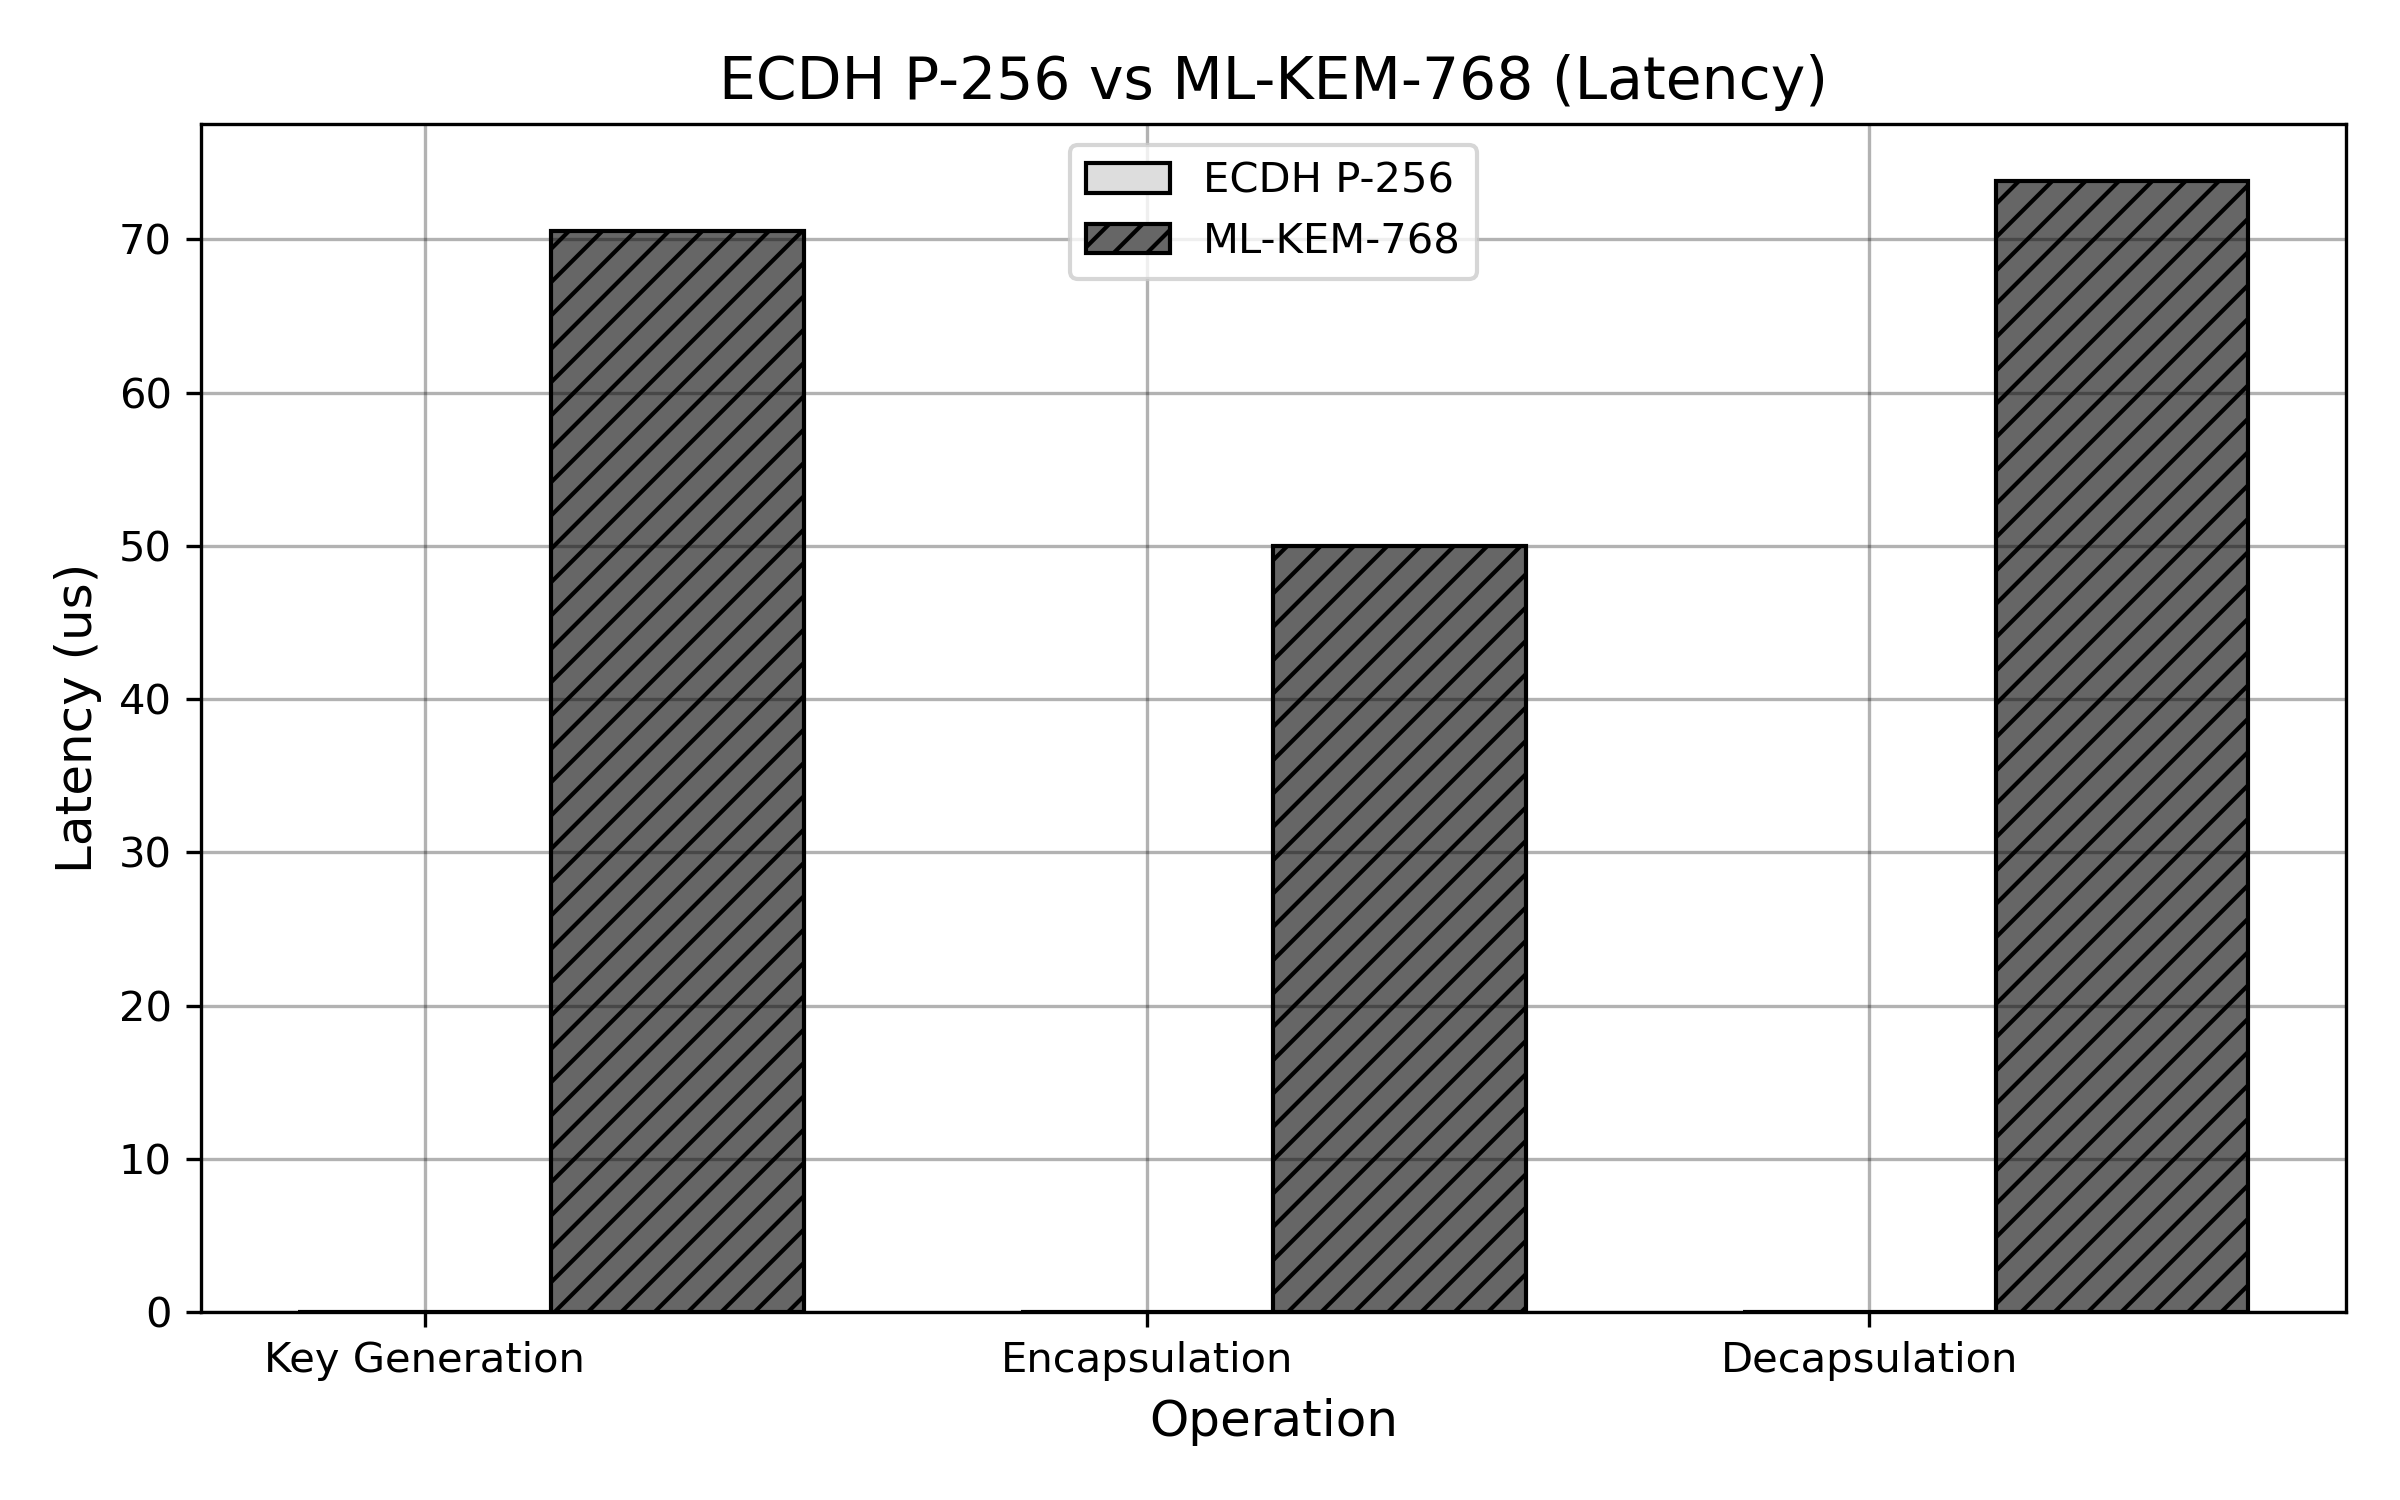
\includegraphics[width=\columnwidth]{plots/exp1_ecdh_vs_mlkem.png}}
\caption{Latency comparison of Key Establishment operations.}
\label{fig:exp1}
\end{figure}

\subsection{Digital Signatures (RSA vs ML-DSA)}
Digital signatures are foundational for code signing and identity verification. We compared RSA-2048 against ML-DSA-65 using a 256-byte payload.

Our benchmarks reveal a massive disparity in key generation times. ML-DSA key generation requires only $212.29~\mu s$, which is over $200\times$ faster than RSA-2048 ($51.8~ms$). 

However, verification—the most common operation in OS contexts—shows the inverse. ML-DSA verification takes $208.24~\mu s$, which is approximately $9\times$ slower than RSA's highly optimized verification ($22.51~\mu s$).

\begin{figure}[htbp]
\centerline{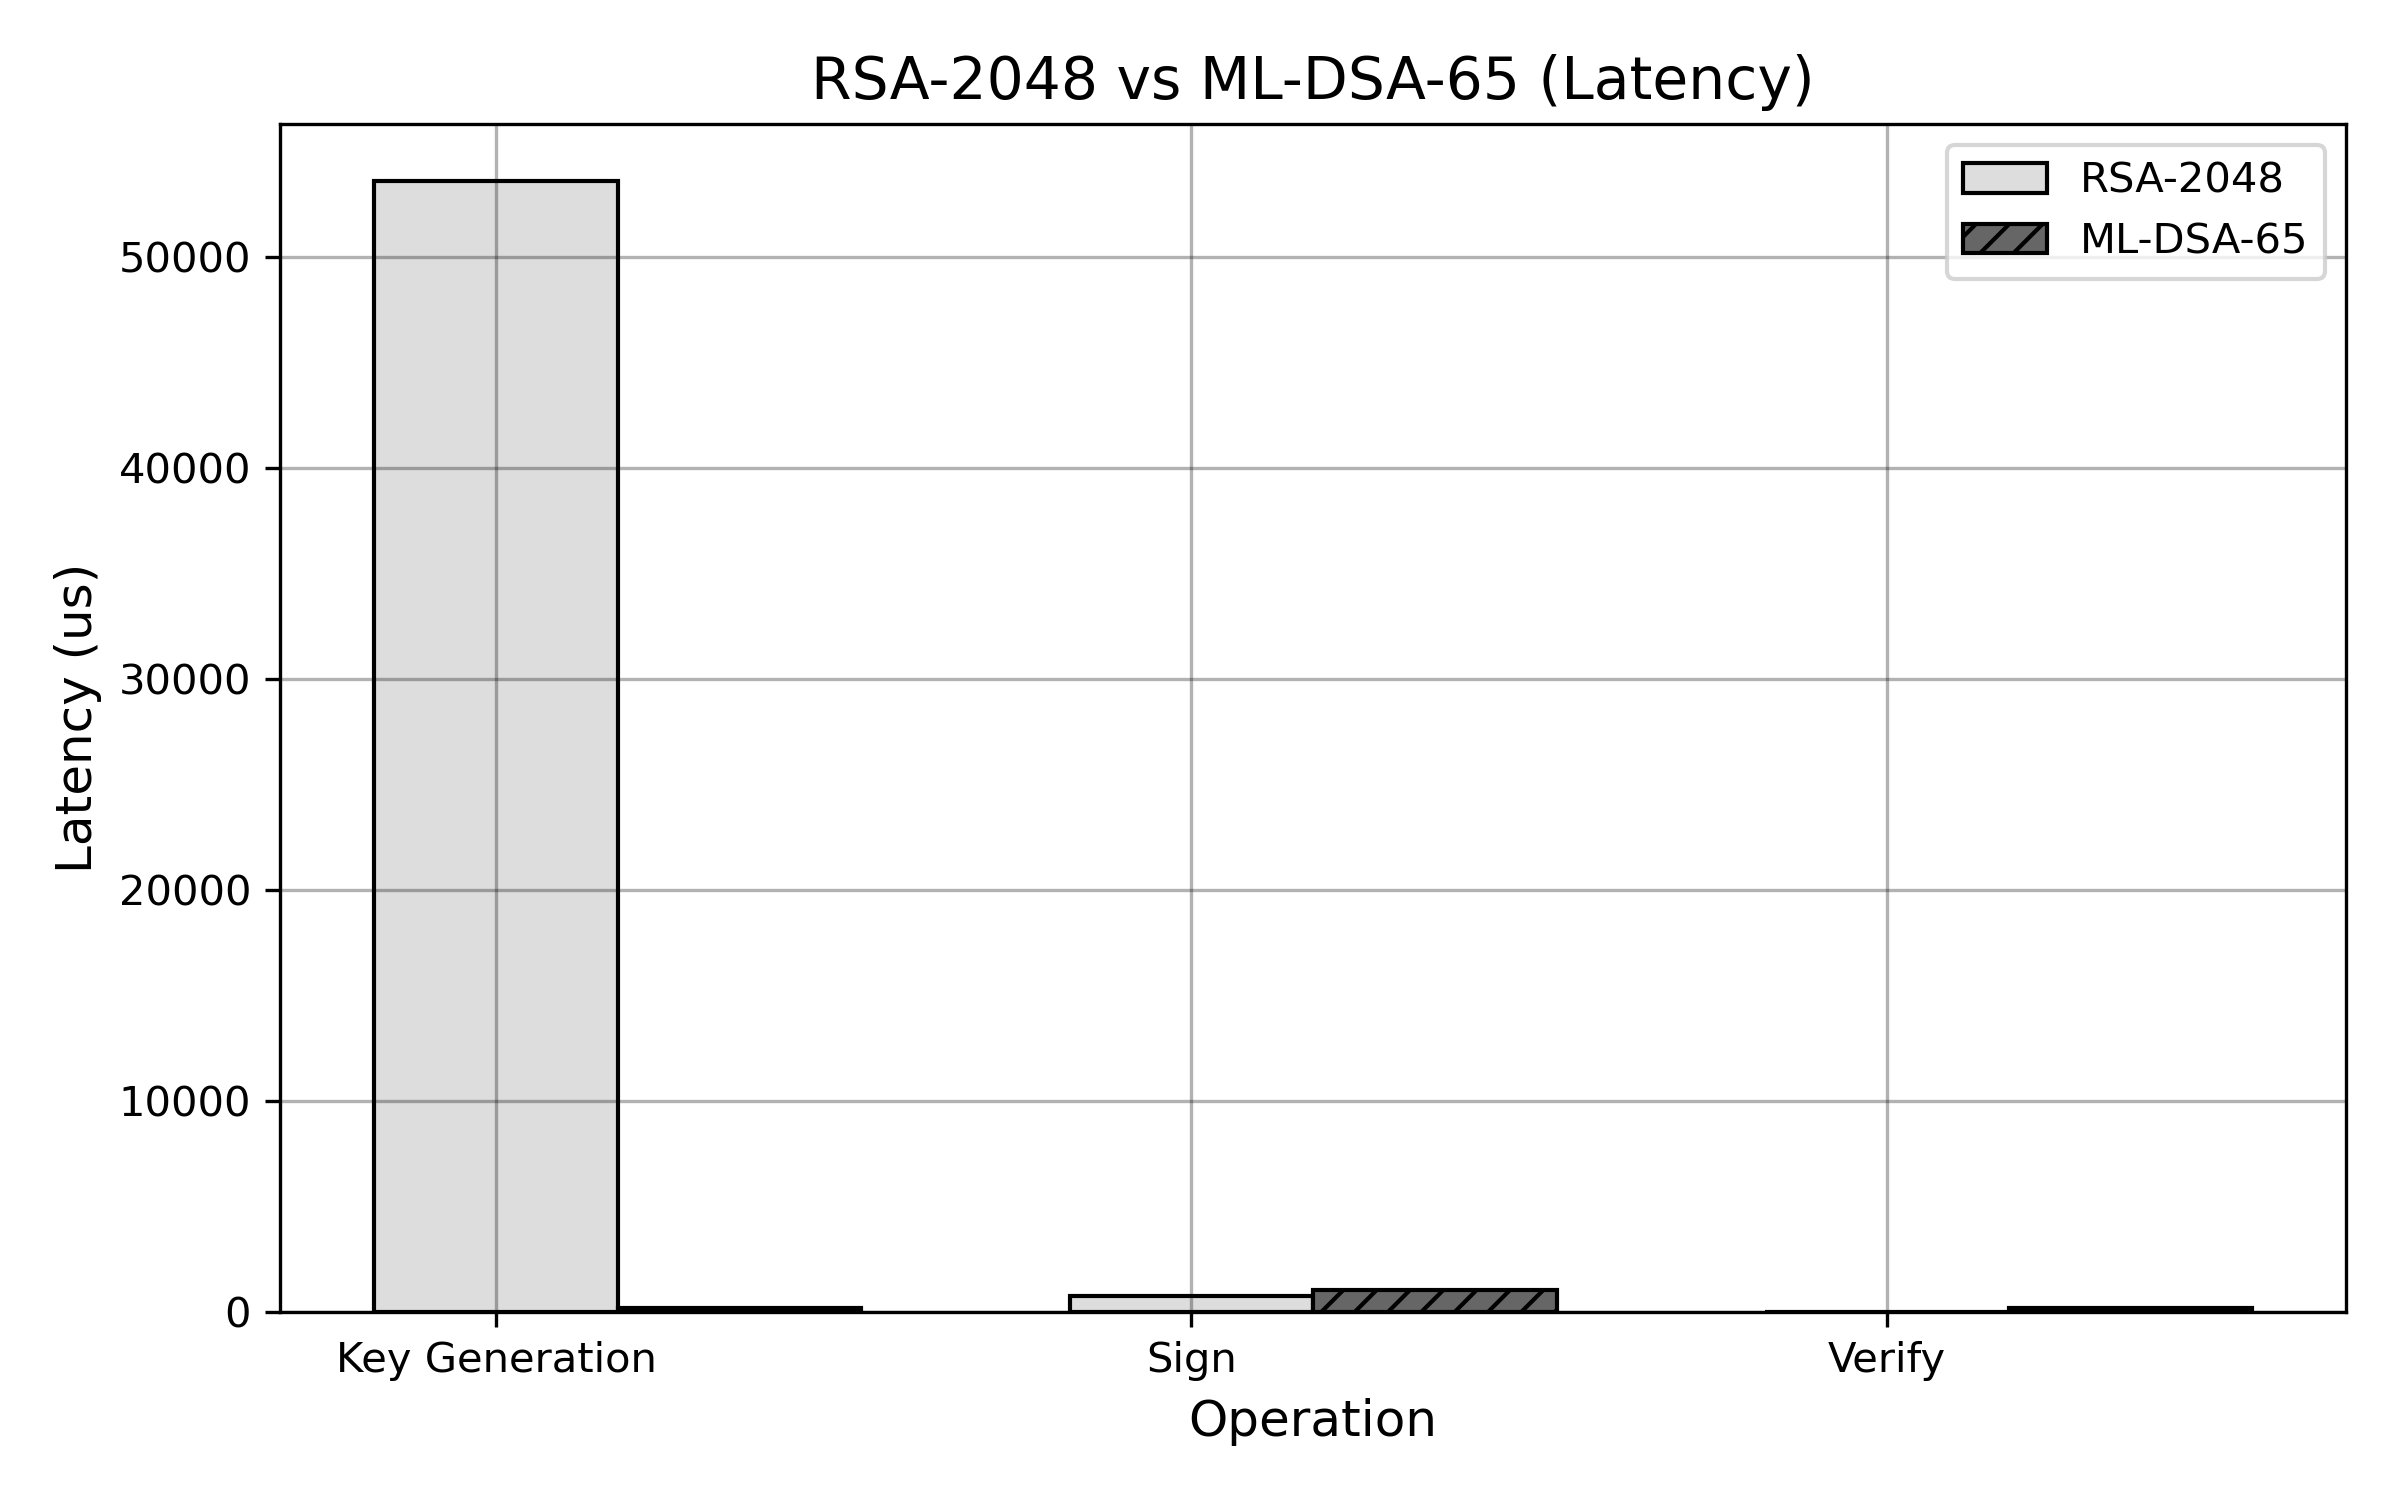
\includegraphics[width=\columnwidth]{plots/exp2_rsa_vs_mldsa.png}}
\caption{Latency comparison of Digital Signature operations.}
\label{fig:exp2}
\end{figure}

\subsection{Secure Boot Simulation}
To understand the practical impact of the slower ML-DSA verification, we simulated a secure boot process verifying a synthetic 4MB kernel image.

\textbf{Insight:} RSA-2048 verified the 4MB kernel in $2.01~ms$. ML-DSA-65 completed the verification in $8.22~ms$. While ML-DSA is $4\times$ slower in this context, the absolute overhead of $\sim 6.2~ms$ is negligible in the context of system boot times, confirming that ML-DSA is perfectly viable for XenevaOS secure boot architecture.

\begin{figure}[htbp]
\centerline{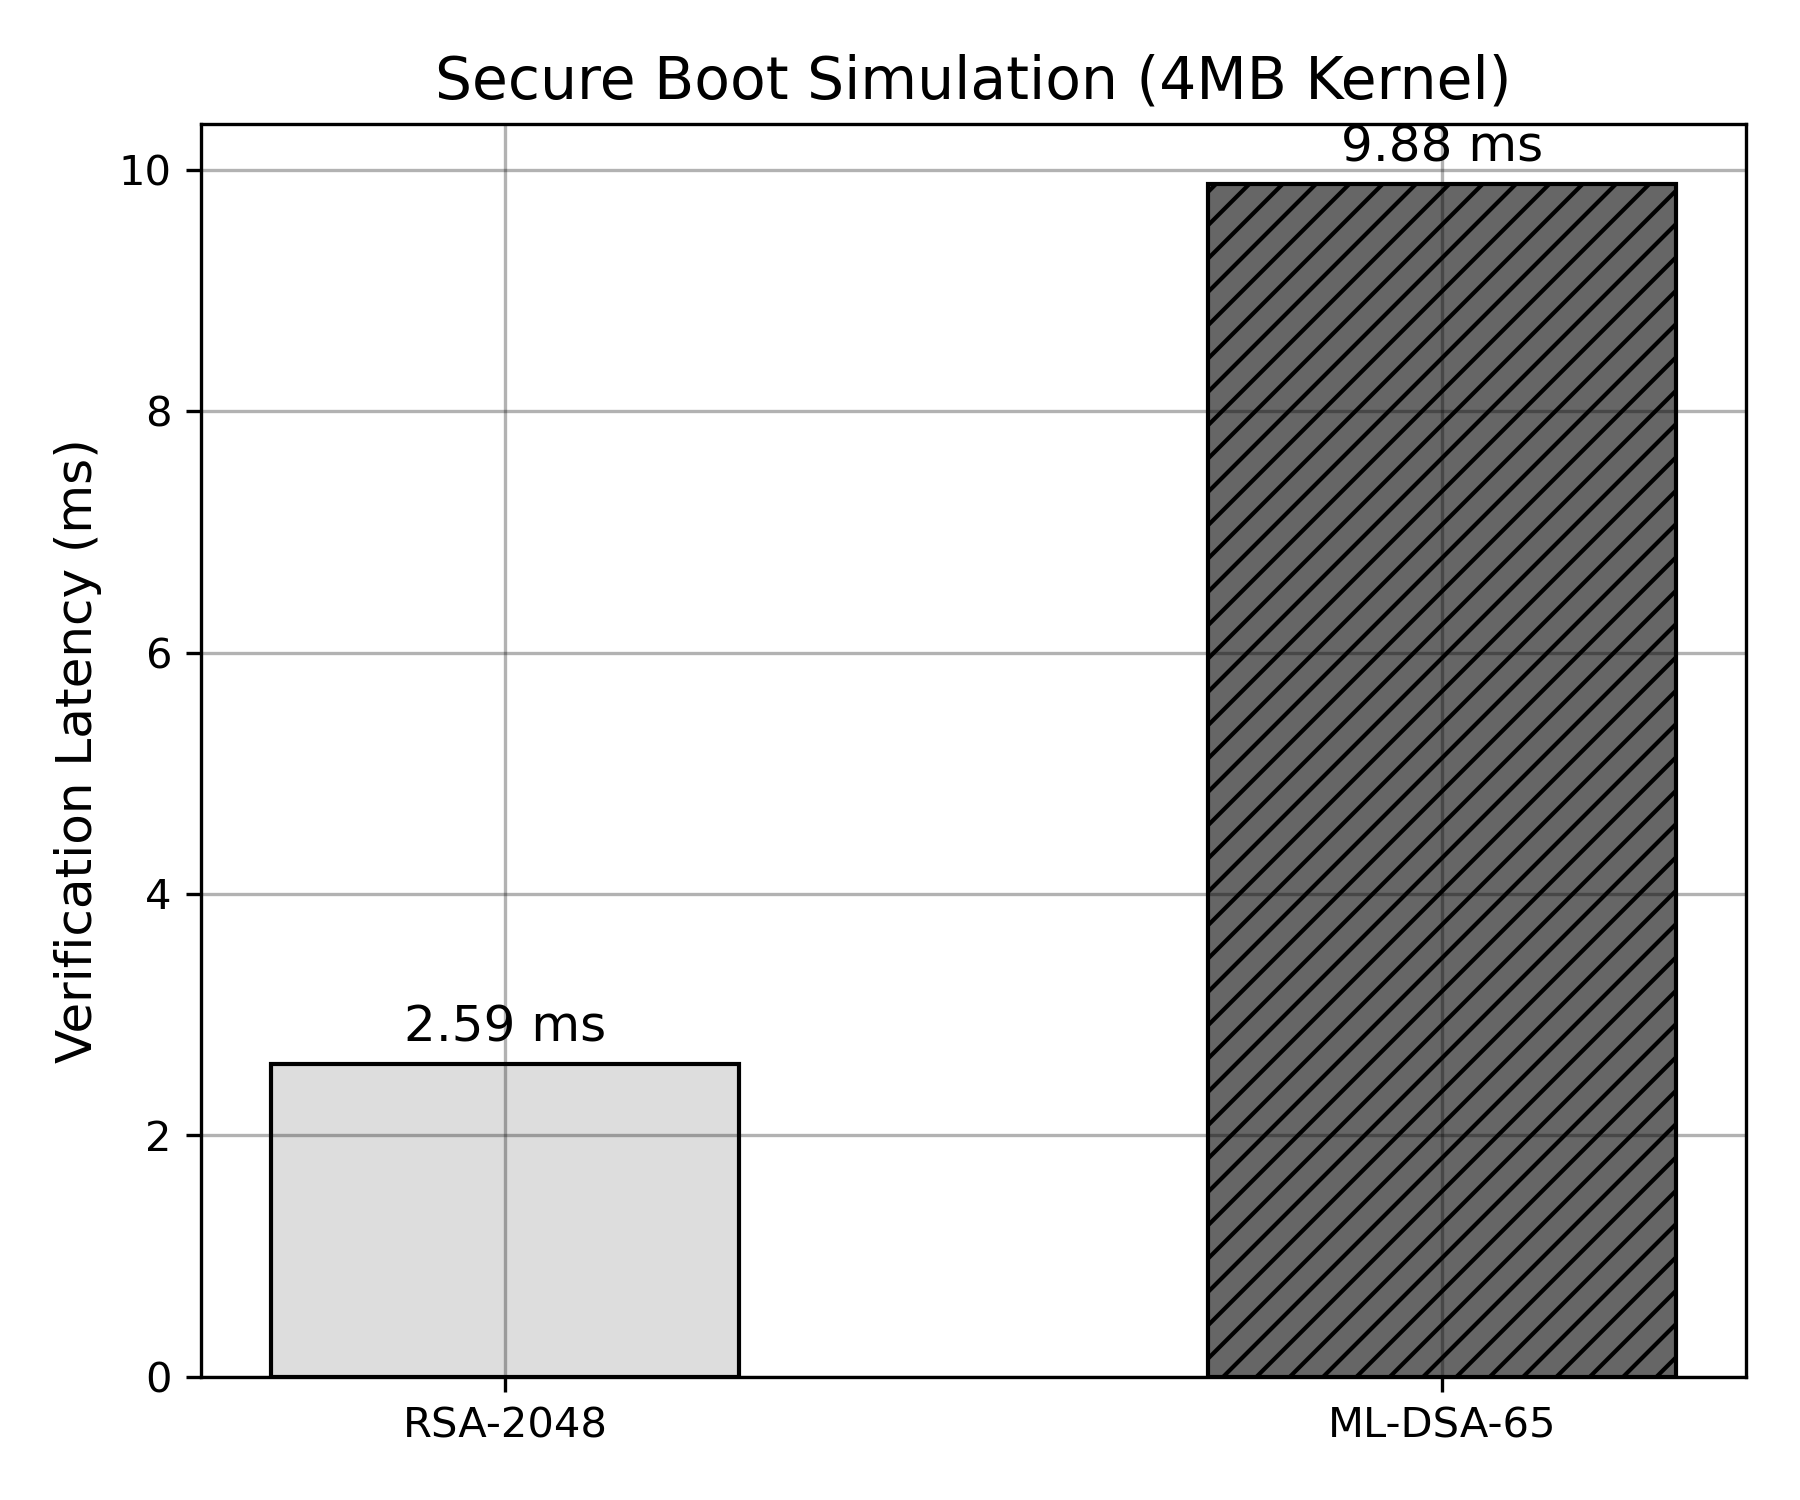
\includegraphics[width=\columnwidth]{plots/exp3_secure_boot.png}}
\caption{Secure Boot Kernel (4MB) Verification Latency.}
\label{fig:exp3}
\end{figure}

\subsection{Secure IPC Simulation}
Process isolation and secure messaging require high-throughput symmetric encryption bootstrapped by asymmetric key exchange. We simulated a full IPC handshake: key generation, Key Derivation (SHA-256), and Authenticated Encryption (AES-256-GCM) on a 4KB payload.

\textbf{Insight:} The Post-Quantum IPC pipeline (ML-KEM + AES) completed the full roundtrip in $114.98~\mu s$ ($8,697$ ops/sec), outperforming the Classical pipeline (ECDH + AES) which took $126.88~\mu s$ ($7,881$ ops/sec). 

The PQC pipeline is roughly \textbf{$9.4\%$ faster} end-to-end. The high speed of lattice-based KEM encapsulation directly outperforms the heavy scalar multiplication required for Elliptic Curve Diffie-Hellman derivation.

\begin{figure}[htbp]
\centerline{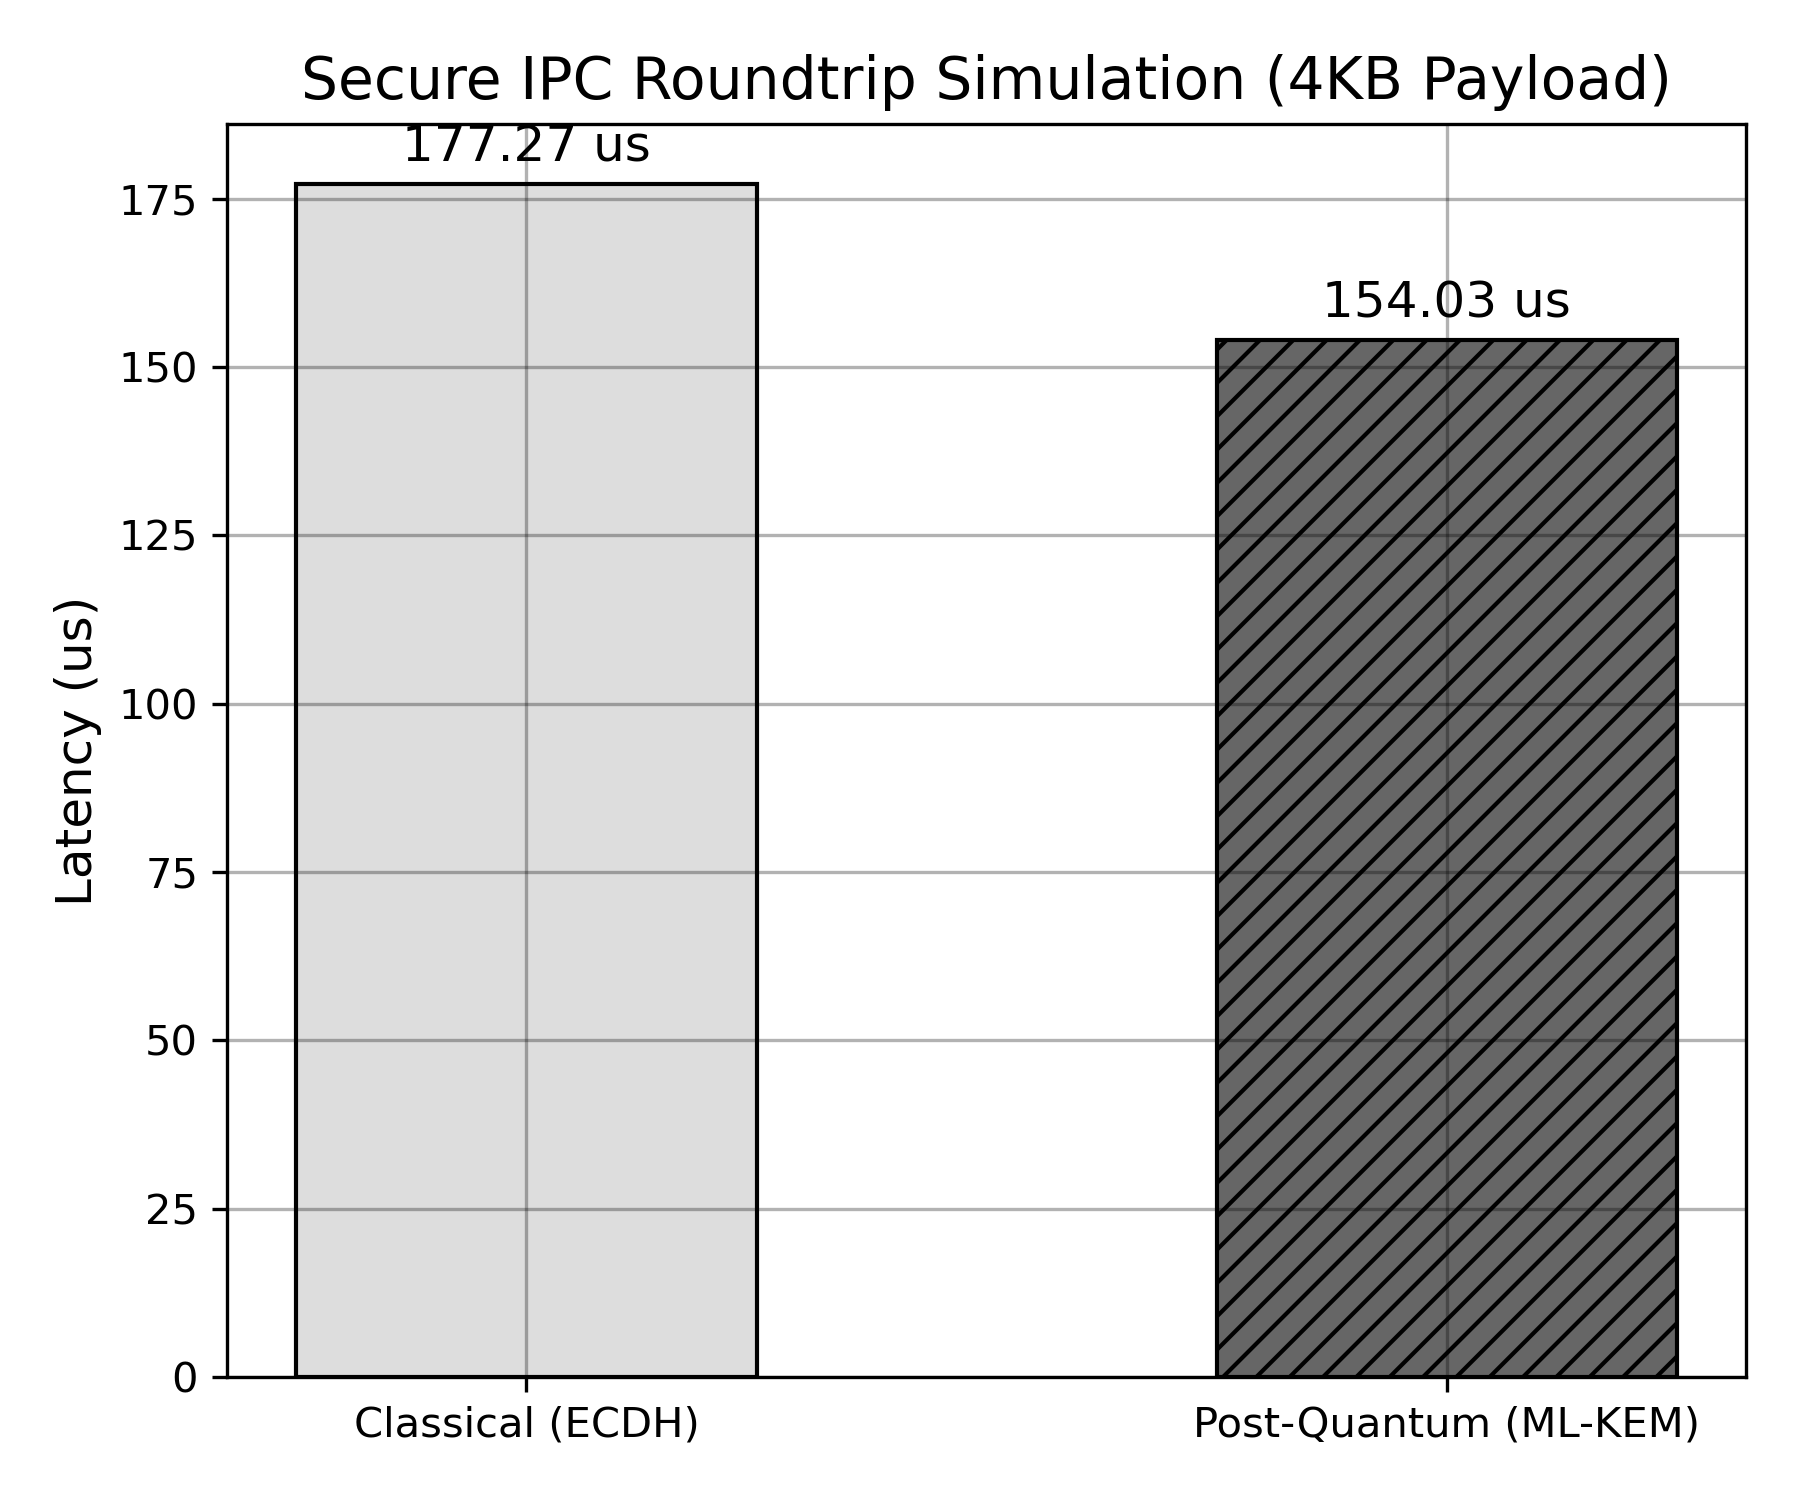
\includegraphics[width=\columnwidth]{plots/exp5_secure_ipc.png}}
\caption{Secure IPC Roundtrip Latency (4KB Payload).}
\label{fig:exp5}
\end{figure}

\section{Conclusion}
The integration of Post-Quantum Cryptography into XenevaOS presents a highly viable path forward. While ML-DSA imposes a theoretical penalty on verification throughput, the absolute real-world impact on operations like secure boot is negligible ($\sim 6~ms$). Furthermore, ML-KEM provides exceptional performance characteristics for transient key exchange, resulting in a measurable performance \textit{increase} for secure IPC handshakes. 

Future work will evaluate the memory and bandwidth impact of larger PQC public keys and signatures within constrained environments.

\end{document}
